\chapter{Решаем задачи в функциональном стиле}
\label{functionally-solving-problems}
\colorbox{lgray}
{
\begin{minipage}{1.0\linewidth}
    Похоже, что мы уже выпили достаточно эрлангового сока, чтобы сделать что\--нибудь полезное.
    В этой главе не будет ничего нового, а просто будет показано как применять элементы увиденного ранее.
    Задачи были взяты из книги Miran\--а \href{http://learnyouahaskell.com/functionally-solving-problems}{Learn You a Haskell}.
    Я использовал те же самые пути решения для того, чтобы любопытный читатель смог сравнивать решения на Erlang и Haskell как ему заблагорассудится.
    Если вы сделаете такое сравнение, то наверняка найдёте, что для двух языков с такими разными синтаксисами, конечные результаты очень похожи.
    Так происходит потому, что изученные концепции функционального программирования относительно легко переносить на другие функциональные языки.
\end{minipage}
}
\section{Калькулятор в обратной польской записи}
\label{reverse-polish-notation-calculator}
Большинство людей научились записывать арифметические выражения, помещая оператор между числами (\ops{(2 + 2) / 5}).
Так вводятся математические выражения в большинстве калькуляторов, и такую запись вас обучили использовать при счёте на школьных уроках. 
У этой записи есть недостаток: вам необходимо знать о порядке вычисления операторов.
Умножение и деление считается более важным (имеет более высокий приоритет), чем сложение и вычитание.

Существует ещё один способ записи, который называется \emph{префиксной записью} или \emph{польской записью}, в которой оператор записывается перед операндами.
В этой записи выражение \ops{(2 + 2) / 5} примет вид \ops{(/ (+ 2 2) 5)}.
Если мы решим, что \ops{+\strut}  и \ops{/\strut} должны всегда принимать два аргумента, то \ops{(/ (+ 2 2) 5)} можно просто записать как \ops{/ + 2 2 5}.

Однако, мы сосредоточимся на \emph{обратной польской записи} (или просто ОПЗ), которая противоположна префиксной записи: в ней оператор следует за операндами.
Тот же самый пример, приведённый выше, в ОПЗ будет записан как \ops{2 2 + 5 /}.
Можно привести и другие примеры: \ops{9 * 5 + 7} и \ops{10 * 2 * (3 + 5) / 2} транслируются соответственно в \ops{9 5 * 7} и \ops{10 2 * 3 4 + * 2 /}.
Эта запись очень широко использовалась в ранних моделях калькуляторов, так как требовала малого количества памяти.
А некоторые люди до сих пор носят с собой калькуляторы с ОПЗ.
Именно такой калькулятор мы и напишем.

Для начала неплохо было бы понять как читаются выражения ОПЗ.
Можно искать операторы один за одним и, учитывая арность, перегруппировывать их с операндами.
\begin{align*}
    &10\;4\;3+2 * -\\
    &10\;(4\;3\; +)\;2 * -\\
    &10\; ((4\; 3\; +)\; 2\; *) -\\ 
    &(10\; ((4\; 3\; +)\; 2\; *) -)\\
    &(10\; (7\; 2\; *) -)\\
    &(10\; 14\; -)\\
    &-4\\
\end{align*}

Но в компьютере или калькуляторе намного проще было бы создать \emph{стек} всех операндов в порядке их расположения.
Возьмём математическое выражение \ops{10 4 3 + 2 * -}.
Первый операнд 10.
Мы добавляем его в стек.
Затем идёт 4.
Его мы тоже кладём на вершину стека.
Третьим идёт число 3.
Мы помещаем в стек и его.
Теперь стек принял следующий вид:
\begin{figure}[h!]
    \centering
    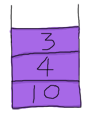
\includegraphics[width=0.12\textwidth]{stack1.png}
\end{figure}

Следующий символ это \ops{+\strut}.
Он представляет собой функцию арности 2.
Чтобы ею воспользоваться, нам необходимо  передать ей два операнда, которые мы извлечём из стека:
\begin{figure}[h!]
    \centering
    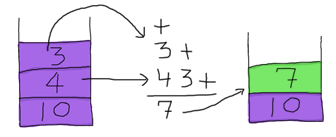
\includegraphics[width=0.4\textwidth]{stack2.png}
\end{figure}

Полученную цифру 7 мы загоняем в верхушку стека (фу, мы же не хотим, чтобы эти грязные числа летали повсюду!)
Теперь стек содержит [7, 10], и от первоначального выражения осталось лишь \ops{2 * -}.
Мы берём 2 и помещаем его в вершину стека.
Затем мы видим операцию \ops{*\strut}, которой для работы необходимо передать два операнда.
И снова мы извлекаем их из стека:
\begin{figure}[h!]
    \centering
    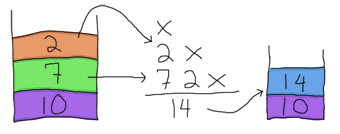
\includegraphics[width=0.4\textwidth]{stack3.png}
\end{figure}

И помещаем 14 в вершину стека.
Остаётся лишь \ops{-\strut}, которому необходимо два операнда.
О, невиданная удача!
В нашем стеке как раз осталось два операнда.
Используем же их!
\begin{figure}[h!]
    \centering
    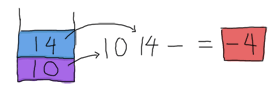
\includegraphics[width=0.4\textwidth]{stack4.png}
\end{figure}

А теперь мы получили результат.
Этот стек\--ориентированный подход относительно дуракоустойчив.
А то, что для начала вычислений требуется парсить мало данных, объясняет почему этот способ годится для старых калькуляторов.
Есть и другие причины для использования ОПЗ, но в этом руководстве они не обсуждаются.
За этим лучше обратиться к \href{http://en.wikipedia.org/wiki/Reverse_Polish_notation}{Статье на Wikipedia}.

Как только мы справились со сложными моментами, записать решение на Erlang становится достаточно просто.
Оказывается, что самое сложное \--- определить шаги для получения конечного результата.
А это мы только что проделали.
Неплохо.
Откройте файл \emph{\href{http://learnyousomeerlang.com/static/erlang/calc.erl}{calc.erl}}.

Первое, о чём стоит побеспокоиться \--- представление математических выражений.
Чтобы упростить задачу мы, наверное, введём их в виде строки: \ops{''10 4 3 + 2 * -''}.
В этой строке есть пробелы, которые не оговорены в нашем решении, но необходимы для работы простого лексического анализатора.
После обработки анализатором неплохо было бы получить список термов вида \ops{[''10'',''4'',''3'',''+'',''2'',''*'',''-'']}.
Оказвыается, что функция \ops{\href{http://erldocs.com/R15B/stdlib/string.html\#tokens/2}{string:tokens/2}} делает именно то, что нам нужно:
\begin{lstlisting}[style=erlang]
1> string:tokens("10 4 3 + 2 * -", " ").
["10","4","3","+","2","*","-"]
\end{lstlisting}
